\documentclass[12pt]{article}

% a template that a friend gave, it's worked well enough for me
% i have added some packages and stuff that have proved useful

\usepackage{fancyhdr}
\usepackage{tipa}
\usepackage{fontspec}
\usepackage{amsfonts}
\usepackage{enumitem}
\usepackage[margin=1in]{geometry}
\usepackage{graphicx}
\usepackage{float}
\usepackage{amsmath}
\usepackage{braket}
\usepackage{amssymb}
\usepackage{booktabs}
\usepackage{hyperref}
\usepackage{mathtools}
\usepackage{xcolor}
\usepackage{float}
\usepackage{algpseudocodex}
\usepackage{titlesec}
\usepackage{bbm}

\pagestyle{fancy}
\fancyhf{} % sets both header and footer to nothing
\lhead{Kevin Sheng}
\setmainfont{Comic Neue}
\renewcommand{\headrulewidth}{1pt}
\setlength{\headheight}{0.75in}
\setlength{\oddsidemargin}{0in}
\setlength{\evensidemargin}{0in}
\setlength{\voffset}{-.5in}
\setlength{\headsep}{10pt}
\setlength{\textwidth}{6.5in}
\setlength{\headwidth}{6.5in}
\setlength{\textheight}{8in}
\renewcommand{\headrulewidth}{0.5pt}
\renewcommand{\footrulewidth}{0.3pt}
\setlength{\textwidth}{6.5in}
\usepackage{setspace}
\usepackage{multicol}
\usepackage{float}
\setlength{\columnsep}{1cm}
\setlength\parindent{24pt}
\usepackage [english]{babel}
\usepackage [autostyle, english = american]{csquotes}
\MakeOuterQuote{"}

\setlength{\parskip}{6pt}
\setlength{\parindent}{0pt}

\titlespacing\section{0pt}{12pt plus 4pt minus 2pt}{0pt plus 2pt minus 2pt}
\titlespacing\subsection{0pt}{12pt plus 4pt minus 2pt}{0pt plus 2pt minus 2pt}
\titlespacing\subsubsection{0pt}{12pt plus 4pt minus 2pt}{0pt plus 2pt minus 2pt}

\hypersetup{colorlinks=true, urlcolor=blue}

\newcommand{\correction}[1]{\textcolor{red}{#1}}

\usepackage{fancyvrb}

\rhead{Math 168}

\DeclareMathOperator{\Fr}{Fr}
\DeclareMathOperator{\Tr}{Tr}
\newcommand{\lra}{\xLeftrightarrow}
\newcommand{\ra}{\xRightarrow}

\setlist[enumerate,1]{label=(\alph*)}

\begin{document}

\section{Gemini Error Correction}

Though the title says $N=11$, there's actually $13$ nodes in the graph,
with some labelled twice. I'm not sure why this is the case,
but worse has happened.

As for the actual cores, the entire graph is also a $2$-core in and of itself.
It's connected, and every node has at least two edges coming out of it.
This invalidates the orange region defined by Gemini, since it isn't maximal.

Also, the graph's $3$-core is every node except $9$, $10$, and $11$,
which is a superset of the red region Gemini highlighted.

\section{Newman 7.9}

\subsection{Part A}

The entire first graph is a $3$-core.
It's connected, and every node has at least degree $3$.

The second graph is a $2$-core in its entirety for similar reasons.
However, it has no $3$-cores.
When we continually eliminate nodes with degree of $2$ or lower,
all the nodes disappear in the order specified in the figure below.
\begin{center}
      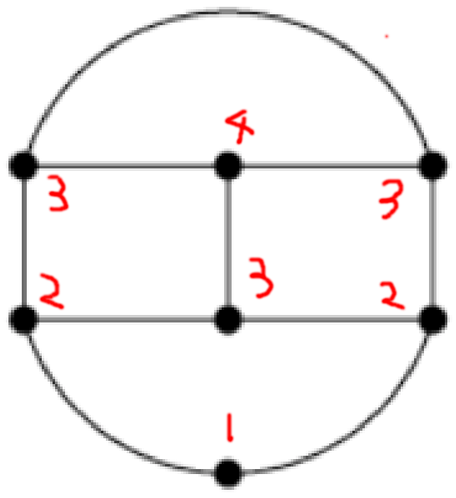
\includegraphics[width=3cm]{img/hw4/core2}
\end{center}

\subsection{Part B}

\begin{enumerate}[label=\roman*.]
      \item This graph is a tree, so for every pair of nodes there's exactly one shortest path.
            Also, all paths must go through the central node.
            Thus, $n_{st}^{v_0}=g_{st}=1$ for all $s$ and $t$, making $x_{v_0}=\boxed{n^2}$.

      \item The peripheral nodes are only on the shortest path when they're
            the start or the destination.
            Thus, there's only $2n-1$ instances of $n_{st}^{v_i}=1$, making $x_{v_i}=\boxed{2n-1}$.

      \item Since this star graph is a tree, there are no triangles.
            Thus, this network does not exhibit any form of triadic closure
            and $C_i=C_{\text{avg}}=0$.
\end{enumerate}

\section{\texorpdfstring{$k$}{k}-regular Networks}

\begin{enumerate}
      \item Every connected $k$-regular network is its own $k$-core by definition.
            It's a connected component, and each node is connected to at least $k$
            other nodes in the core since it has degree $k$.

      \item Consider the following $3$-regular graph:
            \begin{center}
                  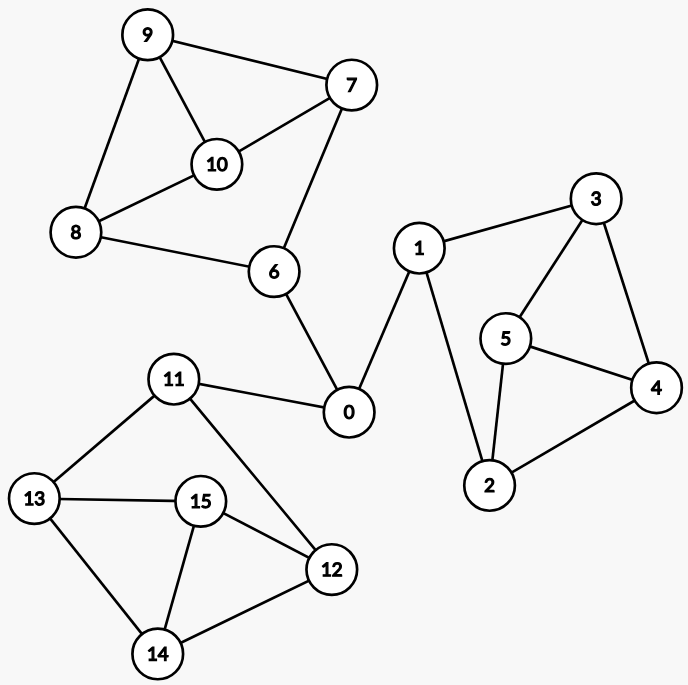
\includegraphics[width=10cm]{img/hw4/not_3_comp}
            \end{center}
            Any path from $1$ to $6$ has to go through $0$, so there can't
            be $3$ node-independent paths between the two nodes.
\end{enumerate}

\pagebreak

\section{Closeness Centrality}

Consider the following 7-node graph:
\begin{center}
      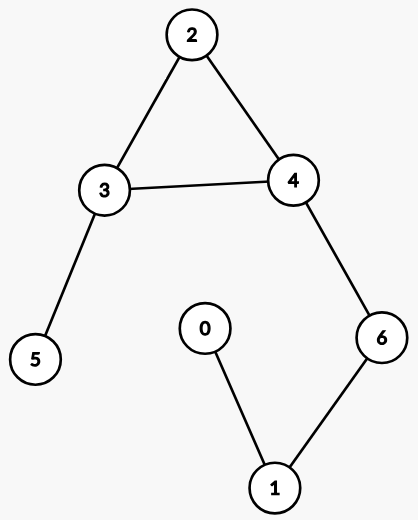
\includegraphics[width=7cm]{img/hw4/closeness}
\end{center}
If we use the first definition of closeness centrality, we have
\begin{gather*}
      C_3=\frac{7}{1+1+1+2+3+4}=\frac{7}{15} \\
      C_6=\frac{7}{1+1+2+2+2+3}=\frac{7}{11}
\end{gather*}
making node $6$ more important.

However, if we use the alternate definition, we get
\begin{gather*}
      C_3=\frac{1}{6}\left(1+1+1+\frac{1}{2}+\frac{1}{3}+\frac{1}{4}\right)=\frac{49}{72} \\
      C_6=\frac{1}{6}\left(1+1+\frac{1}{2}+\frac{1}{2}+\frac{1}{2}+\frac{1}{3}\right)=\frac{23}{36}
\end{gather*}
making node $3$ more important.

(i got this graph by randomly generating ones and checking for inversions lol)

\pagebreak

\section{Similarities}

Here's the code I wrote:
\begin{python}
import networkx as nx
import numpy as np

g = nx.from_edgelist(
    [
        (0, 1),
        (0, 2),
        (1, 2),
        (2, 3),
        (2, 6),
        (3, 4),
        (4, 5),
        (4, 9),
        (5, 6),
        (6, 7),
        (6, 8),
        (7, 8),
        (9, 10),
        (10, 11),
        (10, 12),
        (11, 12),
    ]
)
n = len(g.nodes)

adj = np.zeros((n, n))
for a, b in g.edges:
    adj[a, b] = adj[b, a] = 1

pearson = np.empty((n, n))
cosine = np.empty((n, n))
for i in range(n):
    for j in range(i, n):
        coeff = np.corrcoef(adj[i], adj[j])
        pearson[i, j] = pearson[j, i] = coeff[0, 1]

        dot = adj[i] @ adj[j]
        mags = np.linalg.norm(adj[i]) * np.linalg.norm(adj[j])
        cosine[i, j] = cosine[j, i] = dot / mags

common = adj @ adj
deg = adj @ np.ones((n, 1))
jaccard = common / ((deg + deg.T) - common)

print("COSINE:")
print(np.round(cosine, 2))

print("JACCARD:")
print(np.round(jaccard, 2))

print("PEARSON:")
print(np.round(pearson, 2))
\end{python}

The output of this script is on the next page.

\pagebreak

\begin{Verbatim}[fontsize=\small]
COSINE:
[[1.   0.5  0.35 0.5  0.   0.   0.35 0.   0.   0.   0.   0.   0.  ]
 [0.5  1.   0.35 0.5  0.   0.   0.35 0.   0.   0.   0.   0.   0.  ]
 [0.35 0.35 1.   0.   0.29 0.35 0.   0.35 0.35 0.   0.   0.   0.  ]
 [0.5  0.5  0.   1.   0.   0.5  0.35 0.   0.   0.5  0.   0.   0.  ]
 [0.   0.   0.29 0.   1.   0.   0.29 0.   0.   0.   0.33 0.   0.  ]
 [0.   0.   0.35 0.5  0.   1.   0.   0.5  0.5  0.5  0.   0.   0.  ]
 [0.35 0.35 0.   0.35 0.29 0.   1.   0.35 0.35 0.   0.   0.   0.  ]
 [0.   0.   0.35 0.   0.   0.5  0.35 1.   0.5  0.   0.   0.   0.  ]
 [0.   0.   0.35 0.   0.   0.5  0.35 0.5  1.   0.   0.   0.   0.  ]
 [0.   0.   0.   0.5  0.   0.5  0.   0.   0.   1.   0.   0.5  0.5 ]
 [0.   0.   0.   0.   0.33 0.   0.   0.   0.   0.   1.   0.41 0.41]
 [0.   0.   0.   0.   0.   0.   0.   0.   0.   0.5  0.41 1.   0.5 ]
 [0.   0.   0.   0.   0.   0.   0.   0.   0.   0.5  0.41 0.5  1.  ]]
JACCARD:
[[1.   0.33 0.2  0.33 0.   0.   0.2  0.   0.   0.   0.   0.   0.  ]
 [0.33 1.   0.2  0.33 0.   0.   0.2  0.   0.   0.   0.   0.   0.  ]
 [0.2  0.2  1.   0.   0.17 0.2  0.   0.2  0.2  0.   0.   0.   0.  ]
 [0.33 0.33 0.   1.   0.   0.33 0.2  0.   0.   0.33 0.   0.   0.  ]
 [0.   0.   0.17 0.   1.   0.   0.17 0.   0.   0.   0.2  0.   0.  ]
 [0.   0.   0.2  0.33 0.   1.   0.   0.33 0.33 0.33 0.   0.   0.  ]
 [0.2  0.2  0.   0.2  0.17 0.   1.   0.2  0.2  0.   0.   0.   0.  ]
 [0.   0.   0.2  0.   0.   0.33 0.2  1.   0.33 0.   0.   0.   0.  ]
 [0.   0.   0.2  0.   0.   0.33 0.2  0.33 1.   0.   0.   0.   0.  ]
 [0.   0.   0.   0.33 0.   0.33 0.   0.   0.   1.   0.   0.33 0.33]
 [0.   0.   0.   0.   0.2  0.   0.   0.   0.   0.   1.   0.25 0.25]
 [0.   0.   0.   0.   0.   0.   0.   0.   0.   0.33 0.25 1.   0.33]
 [0.   0.   0.   0.   0.   0.   0.   0.   0.   0.33 0.25 0.33 1.  ]]
PEARSON:
[[ 1.    0.41  0.18  0.41 -0.23 -0.18  0.18 -0.18 -0.18 -0.18 -0.23 -0.18 -0.18]
 [ 0.41  1.    0.18  0.41 -0.23 -0.18  0.18 -0.18 -0.18 -0.18 -0.23 -0.18 -0.18]
 [ 0.18  0.18  1.   -0.28  0.03  0.18 -0.44  0.18  0.18 -0.28 -0.37 -0.28 -0.28]
 [ 0.41  0.41 -0.28  1.   -0.23  0.41  0.18 -0.18 -0.18  0.41 -0.23 -0.18 -0.18]
 [-0.23 -0.23  0.03 -0.23  1.   -0.23  0.03 -0.23 -0.23 -0.23  0.13 -0.23 -0.23]
 [-0.18 -0.18  0.18  0.41 -0.23  1.   -0.28  0.41  0.41  0.41 -0.23 -0.18 -0.18]
 [ 0.18  0.18 -0.44  0.18  0.03 -0.28  1.    0.18  0.18 -0.28 -0.37 -0.28 -0.28]
 [-0.18 -0.18  0.18 -0.18 -0.23  0.41  0.18  1.    0.41 -0.18 -0.23 -0.18 -0.18]
 [-0.18 -0.18  0.18 -0.18 -0.23  0.41  0.18  0.41  1.   -0.18 -0.23 -0.18 -0.18]
 [-0.18 -0.18 -0.28  0.41 -0.23  0.41 -0.28 -0.18 -0.18  1.   -0.23  0.41  0.41]
 [-0.23 -0.23 -0.37 -0.23  0.13 -0.23 -0.37 -0.23 -0.23 -0.23  1.    0.27  0.27]
 [-0.18 -0.18 -0.28 -0.18 -0.23 -0.18 -0.28 -0.18 -0.18  0.41  0.27  1.    0.41]
 [-0.18 -0.18 -0.28 -0.18 -0.23 -0.18 -0.28 -0.18 -0.18  0.41  0.27  0.41  1.  ]]
\end{Verbatim}

\end{document}
